\documentclass[journal]{IEEEtran}
\usepackage[a5paper, margin=10mm, onecolumn]{geometry}
%\usepackage{lmodern} % Ensure lmodern is loaded for pdflatex
\usepackage{tfrupee} % Include tfrupee package

\setlength{\headheight}{1cm} % Set the height of the header box
\setlength{\headsep}{0mm}     % Set the distance between the header box and the top of the text

\usepackage{gvv-book}
\usepackage{gvv}
\usepackage{cite}
\usepackage{amsmath,amssymb,amsfonts,amsthm}
\usepackage{algorithmic}
\usepackage{graphicx}
\usepackage{textcomp}
\usepackage{xcolor}
\usepackage{txfonts}
\usepackage{listings}
\usepackage{enumitem}
\usepackage{mathtools}
\usepackage{gensymb}
\usepackage{comment}
\usepackage[breaklinks=true]{hyperref}
\usepackage{tkz-euclide} 
\usepackage{listings}
% \usepackage{gvv}                                        
\def\inputGnumericTable{}                                 
\usepackage[latin1]{inputenc}                                
\usepackage{color}                                            
\usepackage{array}                                            
\usepackage{longtable}                                       
\usepackage{calc}                                             
\usepackage{multirow}                                         
\usepackage{hhline}                                           
\usepackage{ifthen}                                           
\usepackage{lscape}
\begin{document}

\bibliographystyle{IEEEtran}
\vspace{3cm}
\title{Digital Clock}
\author{EE24BTECH11025 - GEEDI HARSHA}
% \maketitle
% \newpage
{\let\newpage\relax\maketitle}

\renewcommand{\thefigure}{\theenumi}
\renewcommand{\thetable}{\theenumi}
\setlength{\intextsep}{10pt} % Space between text and floats


\numberwithin{equation}{enumi}
\numberwithin{figure}{enumi}
\renewcommand{\thetable}{\theenumi}

\section{Introduction}
In this experiment, we designed and implemented a digital clock using six seven-segment displays, an ATmega Arduino, and the IC 7447 decoder. The system supports three modes: Clock, Timer, and Stopwatch. The seven-segment displays are controlled using the IC 7447, which converts binary-coded decimal (BCD) inputs into signals that drive the displays. The Arduino manages the timing, mode switching, and display updates. The project demonstrates the use of interrupts, button inputs, and multiplexing for efficient display control.

\section{Components Used}
The following components were used in this experiment:
\begin{itemize}
    \item 6 Seven-Segment Displays (Common Cathode)
    \item 6 Resistors (220\,$\Omega$)
    \item Wires and Jumper Wires
    \item 1 ATmega Arduino
    \item 1 IC 7447 (BCD to Seven-Segment Decoder)
    \item 1 Breadboard
    \item Power Source 
\end{itemize}


\section{Circuit Design}

The circuit was designed as follows:
\section{Procedure}

\subsection*{1. Hardware Setup}
\begin{itemize}
    \item Connect common-anode 7-segment displays to ATmega328P via breadboard.
    \item Assign segment lines: \texttt{PD2-PD7, PB0} (a-g).
    \item Assign digit select lines: \texttt{A0-A2 (PC0-PC2), 10-12 (PB2-PB4)}.
    \item Connect push buttons to \texttt{PB1, PB5, PC3-PC5} for input control.
    \item Any ports can be used if corresponding code changes are made.
\end{itemize}

\subsection*{2. Software Implementation}
\begin{itemize}
    \item \texttt{seg\_map}: Lookup table for digit display.
    \item \texttt{set\_segments}: Lights up correct segments.
    \item \texttt{enable\_digit}: Disables all digits before enabling the correct one.
    \item \texttt{ISR(TIMER1\_COMPA\_vect)}: Increments time and handles rollovers.
    \item \texttt{check\_buttons}: Enables time adjustments when \texttt{set\_mode = 1}.
    \item \texttt{main}: Configures pins, enables pull-ups, sets 1s interrupts, and runs multiplexing loop.
\end{itemize}


% Table 1: IC 7447 Output to Seven-Segment Display Connections
\begin{table}[h]
    \centering
    \begin{tabular}{|c|c|c|c|c|c|c|c|}
        \hline
        \textbf{7447} & $\bar{a}$ & $\bar{b}$ & $\bar{c}$ & $\bar{d}$ & $\bar{e}$ & $\bar{f}$ & $\bar{g}$ \\ \hline
        \textbf{Display} & a & b & c & d & e & f & g \\ \hline
    \end{tabular}
\end{table}

% Table 2: IC 7447 Input to Arduino Digital Pin Connections
\begin{table}[h]
    \centering
    \begin{tabular}{|c|c|c|c|c|}
        \hline
        \textbf{7447} & D & C & B & A \\ \hline
        \textbf{Arduino} & 5 & 4 & 3 & 2 \\ \hline
    \end{tabular}
\end{table}

\begin{figure}[h]
    \centering
    \begin{minipage}{0.48\textwidth}
        \centering
        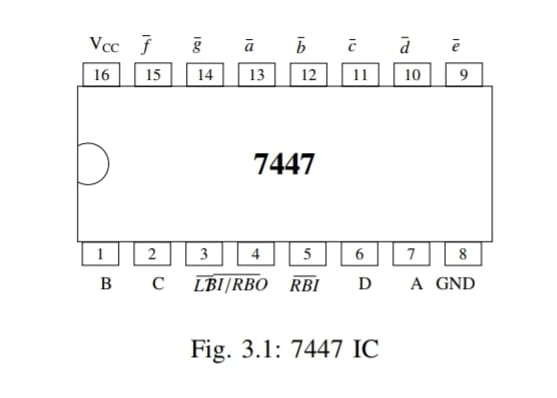
\includegraphics[width=\textwidth]{figs/7447.jpeg} 
    \end{minipage}
    \hfill
    \begin{minipage}{0.48\textwidth}
        \centering
        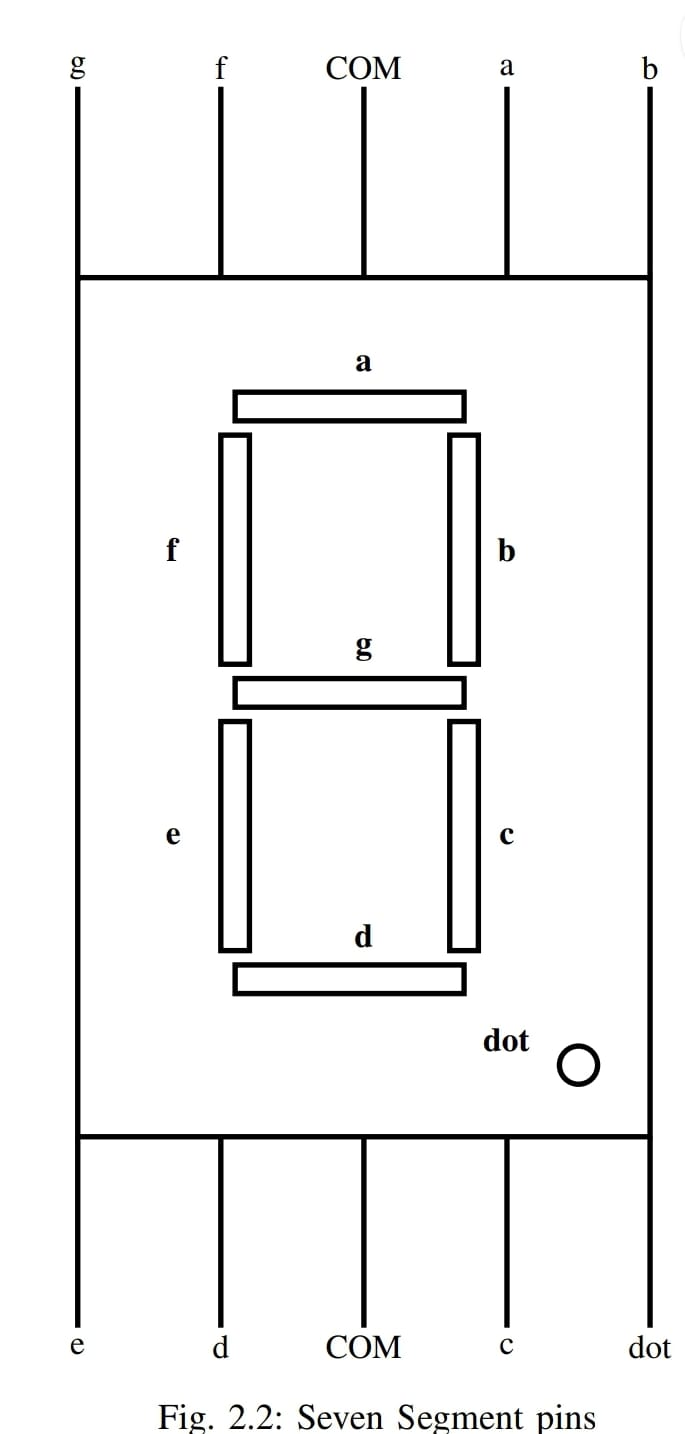
\includegraphics[width=\textwidth]{figs/seven_segment.jpeg}
    \end{minipage}
\end{figure}
\subsection*{1. Power Supply}
\begin{itemize}
    \item Arduino \texttt{5V} pin connects to \texttt{V\textsubscript{CC}} of 7447 IC.
    \item Common ground between Arduino and 7447.
\end{itemize}

\subsection*{2. Display Interface}
\begin{itemize}
    \item COM pins of 7-segment displays connect to \texttt{220$\Omega$} resistors, then to Arduino analog pins.
\end{itemize}

\section*{Push Button Functions}
Four tactile switches are connected to digital pins \texttt{6--9}:

\begin{table}[h]
    \centering
    \renewcommand{\arraystretch}{1.2}
    \begin{tabular}{c c l}
        Button & Pin & Function \\
        1 & \texttt{6} & Hour adjust (\texttt{0} to \texttt{23}, then resets). \\
        2 & \texttt{7} & Minute adjust (\texttt{0} to \texttt{59}, then resets). \\
        3 & \texttt{8} & Mode toggle (switches between clock and stopwatch). \\
        4 & \texttt{9} & Pause/resume (halts clock or stopwatch). \\
    \end{tabular}
\end{table}



\newpage



\section{Code}
The Arduino code for controlling the digital clock, timer, and stopwatch is provided below:

\begin{lstlisting}[language=C++, caption={Arduino Code for Digital Clock, Timer, and Stopwatch}]
#define F_CPU 16000000UL
#include <avr/io.h>
#include <util/delay.h>
#include <avr/interrupt.h>

#define BCD_PORT PORTD
#define BCD_DDR DDRD
#define BCD_MASK 0b00111100  // PD2 to PD5

#define COMMON_PORT PORTC
#define COMMON_DDR DDRC

#define MODE_BUTTON PB0 // Switch between Clock, Timer, and Stopwatch
#define STOPWATCH_BUTTON PB1 // Start/Stop Stopwatch and Timer

volatile int seconds = 0, minutes = 30, hours = 15;
volatile int timer_seconds = 0, timer_minutes = 0, timer_hours = 0;
volatile int stopwatch_seconds = 0, stopwatch_minutes = 0, stopwatch_hours = 0;
volatile int mode = 0; // 0 = Clock, 1 = Timer, 2 = Stopwatch
volatile int stopwatch_running = 0; // 1 = Running, 0 = Stopped

void setup() {
    // Set BCD display pins (PD2-PD5) as output
    BCD_DDR |= BCD_MASK;
    BCD_PORT &= ~BCD_MASK;

    // Set digit selector pins (PORTC) as output
    COMMON_DDR = 0xFF;
    COMMON_PORT = 0x00;

    // Enable pull-up resistors for buttons
    PORTD |= (1 << PD6) | (1 << PD7);
    PORTB |= (1 << MODE_BUTTON) | (1 << STOPWATCH_BUTTON);

    // Timer1 Setup: CTC Mode, 1-second interval
    TCCR1B |= (1 << WGM12) | (1 << CS12) | (1 << CS10);
    OCR1A = 15625; // 1-second interrupt
    TIMSK1 |= (1 << OCIE1A);

    // Debug LED on PC7 (Bit 7 of PORTC) to check if ISR is running
    DDRC |= (1 << 7);  // Set PC7 as output
    PORTC &= ~(1 << 7); // Initially turn it off

    sei(); // Enable global interrupts
}

ISR(TIMER1_COMPA_vect) {
    PORTC ^= (1 << 7); // Toggle PC7 to check ISR is running

    // Clock Mode Updates
    if (mode == 0) {
        seconds++;
        if (seconds == 60) {
            seconds = 0;
            minutes++;
            if (minutes == 60) {
                minutes = 0;
                hours = (hours + 1) % 24;
            }
        }
    }

    // Timer Countdown (only when running)
    if (mode == 1 && stopwatch_running) {  
        if (timer_seconds > 0 || timer_minutes > 0 || timer_hours > 0) {
            if (timer_seconds == 0) {
                if (timer_minutes > 0) {
                    timer_minutes--;
                    timer_seconds = 59;
                } else if (timer_hours > 0) {
                    timer_hours--;
                    timer_minutes = 59;
                    timer_seconds = 59;
                }
            } else {
                timer_seconds--;
            }
        }
    }

    // Stopwatch Increment
    if (mode == 2 && stopwatch_running) {
        stopwatch_seconds++;
        if (stopwatch_seconds == 60) {
            stopwatch_seconds = 0;
            stopwatch_minutes++;
            if (stopwatch_minutes == 60) {
                stopwatch_minutes = 0;
                stopwatch_hours = (stopwatch_hours + 1) % 24;
            }
        }
    }
}

void displayTime();
void setBCD(int value);
void checkButtons();

int main() {
    setup();
    while (1) {
        checkButtons();
        displayTime();
    }
}

// Function to display time on a 6-digit 7-segment display
void displayTime() {
    int digits[6];

    if (mode == 0) { // Clock Mode
        digits[0] = hours / 10;
        digits[1] = hours % 10;
        digits[2] = minutes / 10;
        digits[3] = minutes % 10;
        digits[4] = seconds / 10;
        digits[5] = seconds % 10;
    } else if (mode == 1) { // Timer Mode
        digits[0] = timer_hours / 10;
        digits[1] = timer_hours % 10;
        digits[2] = timer_minutes / 10;
        digits[3] = timer_minutes % 10;
        digits[4] = timer_seconds / 10;
        digits[5] = timer_seconds % 10;
    } else { // Stopwatch Mode
        digits[0] = stopwatch_hours / 10;
        digits[1] = stopwatch_hours % 10;
        digits[2] = stopwatch_minutes / 10;
        digits[3] = stopwatch_minutes % 10;
        digits[4] = stopwatch_seconds / 10;
        digits[5] = stopwatch_seconds % 10;
    }

    // Multiplex 7-segment display
    for (int i = 0; i < 6; i++) {
        setBCD(digits[i]); // Send the BCD value first
        COMMON_PORT = (1 << i); // Enable the corresponding digit
        _delay_us(500); // Short delay for smooth display
    }
}

// Function to set BCD output for 7-segment display
void setBCD(int value) {
    BCD_PORT = (BCD_PORT & ~BCD_MASK) | ((value << 2) & BCD_MASK);
}

// Function to check button inputs and update mode/settings
void checkButtons() {
    if (!(PIND & (1 << PD6))) {
        _delay_ms(50);
        if (!(PIND & (1 << PD6))) {
            if (mode == 0) {
                hours = (hours + 1) % 24;
                seconds = 0;
            } else if (mode == 1) {
                timer_hours = (timer_hours + 1) % 24;
                seconds = 0;
            }
            while (!(PIND & (1 << PD6))); // Wait for release
        }
    }

    if (!(PIND & (1 << PD7))) {
        _delay_ms(50);
        if (!(PIND & (1 << PD7))) {
            if (mode == 0) {
                minutes = (minutes + 1) % 60;
                seconds = 0;
            } else if (mode == 1) {
                timer_minutes = (timer_minutes + 1) % 60;
                seconds = 0;
            }
            while (!(PIND & (1 << PD7))); // Wait for release
        }
    }

    if (!(PINB & (1 << MODE_BUTTON))) {
        _delay_ms(50);
        if (!(PINB & (1 << MODE_BUTTON))) {
            mode = (mode + 1) % 3; // Cycle through Clock, Timer, and Stopwatch
            while (!(PINB & (1 << MODE_BUTTON))); // Wait for release
        }
    }

    // Modified section: Stopwatch button controls both Timer and Stopwatch
    if (!(PINB & (1 << STOPWATCH_BUTTON))) {
        _delay_ms(50);
        if (!(PINB & (1 << STOPWATCH_BUTTON))) {
            if (mode == 2) {  // Toggle Stopwatch running
                stopwatch_running = !stopwatch_running;
            } else if (mode == 1) {  // Toggle Timer running
                stopwatch_running = !stopwatch_running;  // Reuse the same flag
            }
            while (!(PINB & (1 << STOPWATCH_BUTTON))) {
                _delay_ms(10);
            }
        }
    }
}
\end{lstlisting}

\section{Code Explanation}
The code is divided into several key sections, each handling a specific functionality of the digital clock, timer, and stopwatch.

\subsection{BCD and Digit Selection}
\begin{itemize}
    \item The BCD output is generated using the \texttt{setBCD()} function, which takes a digit (0-9) and sets the corresponding BCD bits on PORTD (PD2-PD5).
    \item The \texttt{displayTime()} function splits the time into individual digits and uses multiplexing to display them on the six seven-segment displays. Each digit is displayed for a short duration (\texttt{\_delay\_us(500)}) to create the illusion of simultaneous display.
\end{itemize}

\subsection{Button Configuration}
\begin{itemize}
    \item Two buttons are used: one for mode selection (\texttt{MODE\_BUTTON}) and one for controlling the stopwatch/timer (\texttt{STOPWATCH\_BUTTON}).
    \item The \texttt{checkButtons()} function debounces the buttons and handles their actions:
    \begin{itemize}
        \item \texttt{MODE\_BUTTON} cycles through the three modes: Clock, Timer, and Stopwatch.
        \item \texttt{STOPWATCH\_BUTTON} starts/stops the stopwatch or timer depending on the current mode.
    \end{itemize}
\end{itemize}

\subsection{Time Tracking Variables}
\begin{itemize}
    \item Three sets of variables track time for the clock, timer, and stopwatch:
    \begin{itemize}
        \item \texttt{hours}, \texttt{minutes}, \texttt{seconds} for the clock.
        \item \texttt{timer\_hours}, \texttt{timer\_minutes}, \texttt{timer\_seconds} for the timer.
        \item \texttt{stopwatch\_hours}, \texttt{stopwatch\_minutes}, \texttt{stopwatch\_seconds} for the stopwatch.
    \end{itemize}
    \item The \texttt{mode} variable determines which set of variables is currently active.
\end{itemize}

\subsection{Interrupt-Driven Time Updates}
The Timer1 interrupt is configured to trigger every second. The ISR (\texttt{TIMER1\_COMPA\_vect}) handles time updates based on the current mode:
\begin{itemize}
    \item \textbf{Clock Mode:} Increments seconds, minutes, and hours, resetting them as necessary.
    \item \textbf{Timer Mode:} Decrements the timer variables, stopping when all reach zero.
    \item \textbf{Stopwatch Mode:} Increments the stopwatch variables, similar to the clock.
\end{itemize}

\section{Results}
The digital clock successfully displayed the time in the format HH:MM:SS. The system seamlessly switched between Clock, Timer, and Stopwatch modes using the buttons. The seven-segment displays were updated every second, and the circuit operated as expected. The resistors ensured that the displays were not damaged by excessive current.

\section{Conclusion}
This experiment demonstrated the use of seven-segment displays, the IC 7447 decoder, and an ATmega Arduino to create a functional digital clock with additional timer and stopwatch features. The project provided valuable insights into BCD encoding, multiplexing, interrupt handling, and button input processing. Future improvements could include adding a real-time clock (RTC) module for more accurate timekeeping and implementing additional features like alarms or date display.
\begin{thebibliography}{9}

\bibitem{ai_suggestions} AI Suggestions, Personal& Classmates(EE-026,EE-035) Recommendations.

\bibitem{hardware_guide} Hardware Connections Guide, Available from online sources.

\end{thebibliography}
\end{document}


































































